\documentclass[border=4pt]{standalone}
\usepackage{amsmath}
\usepackage{tikz}
\usetikzlibrary{arrows.meta,patterns}

\begin{document}
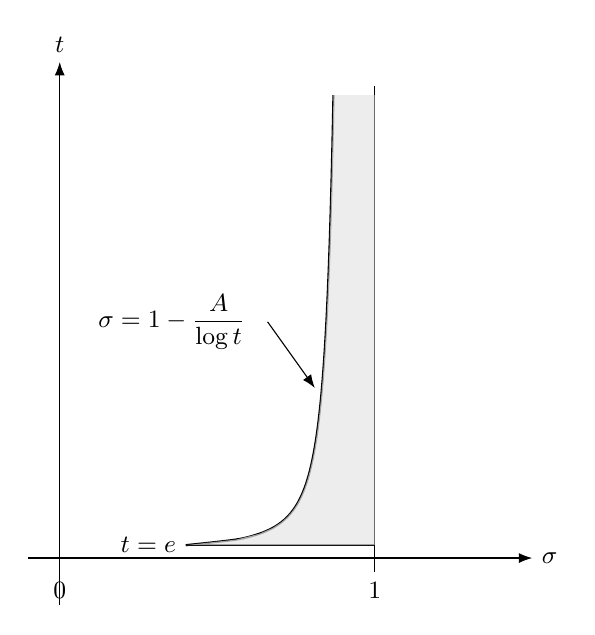
\begin{tikzpicture}[>=Latex, x=4cm, y=0.06cm]
    % axes
    \draw[->] (-0.1,0) -- (1.5,0) node[right] {\small $\sigma$};
    \draw[->] (0,-10) -- (0,105) node[above] {\small $t$};

    % line sigma = 1
    \draw (1,-3) -- (1,100);
    \node[below] at (1,-3) {\small $1$};
    \node[below] at (0,-3) {\small $0$};

    % curve sigma = 1 - A/log t, from t = e upward
    \draw[thick,domain=2.718:98,samples=80,smooth,variable=\t]
        plot ({1-0.6/ln(\t)},{\t});
    % horizontal segment at t = e
    \draw[thick] (0.4,2.718) -- (1,2.718);
    \fill[gray!20,opacity=0.7]
        plot[domain=2.718:98,samples=80,variable=\t] ({1-0.6/ln(\t)},{\t})
        -- (1,98) -- (1,2.718) -- cycle;
    \node[left] at (0.4,2.718) {\small $t=e$};
    \node[left] at (0.62,50) {\small $\sigma=1-\dfrac{A}{\log t}$};
    \draw[->] (0.66,50) -- (0.81,36);
\end{tikzpicture}
\end{document}
